
\documentclass[12pt,a4paper]{article}

% ------------------------------------------------------------
% Fonts & layout
% ------------------------------------------------------------
\usepackage[T1]{fontenc}
\usepackage[utf8]{inputenc}
\usepackage{lmodern}
\usepackage{microtype}
\usepackage{geometry}
\geometry{margin=1in}
\usepackage{array}
\usepackage{booktabs}
\usepackage[table]{xcolor}
\usepackage{tikz}
\usetikzlibrary{positioning}

% ------------------------------------------------------------
% Math
% ------------------------------------------------------------
\usepackage{amsmath,amssymb,amsthm,mathtools}

% Standard operators
\DeclareMathOperator{\id}{id}
\DeclareMathOperator{\im}{im}
\DeclareMathOperator{\coker}{coker}
\DeclareMathOperator{\Hom}{Hom}

\DeclareMathOperator{\Spec}{Spec}
\DeclareMathOperator{\Proj}{Proj}

% Categories / notation
\newcommand{\Ab}{\mathbf{Ab}}
\newcommand{\PreSh}{\mathbf{PreSh}}
\newcommand{\Sh}{\mathbf{Sh}}

\newcommand{\F}{\mathcal F}


% basic number sets
\newcommand{\RR}{\mathbb{R}}

% sheaf letters

\newcommand{\G}{\mathcal G}

\newcommand{\GG}{\mathbb G}


\newcommand{\AffSch}{\mathbf{AffSch}}
\newcommand{\ZZ}{\mathbb Z}

\newcommand{\PP}{\mathbb P}

\usepackage{tikz}
\usetikzlibrary{decorations.pathreplacing}
\usetikzlibrary{positioning,arrows.meta}

% sheaf of continuous real-valued functions
\newcommand{\Czero}{\mathcal C^0}        % “C^0”
\newcommand{\CzeroX}{\mathcal C^0_X}     % sheaf on X (optional)

\newcommand{\Cinfty}{\mathcal C^\infty}
\newcommand{\CinftyM}{\mathcal C^\infty_M} % if you use C^\infty_M

% number sets / standard symbols
\newcommand{\CC}{\mathbb{C}}

% structure sheaf notation in complex geometry
\newcommand{\OO}{\mathcal{O}}
\newcommand{\OOX}{\mathcal{O}_X} % optional convenience



\newcommand{\Sch}{\mathrm{Sch}}
\newcommand{\Rings}{\mathrm{Rings}}

\newcommand{\kappares}{\kappa}
\newcommand{\GammaX}{\Gamma(X,\mathcal O_X)}

\newtheorem{theorem}{Theorem}[section]
\newtheorem{proposition}[theorem]{Proposition}
\newtheorem{lemma}[theorem]{Lemma}

\newcommand{\nilrad}{\sqrt{(0)}}

\newcommand{\Frac}{\operatorname{Frac}}
\newcommand{\codim}{\operatorname{codim}}
\newcommand{\trdeg}{\operatorname{trdeg}}

\newcommand{\height}{\operatorname{height}}

\newcommand{\Pic}{\operatorname{Pic}}
\newcommand{\divisor}{\operatorname{div}}

\newcommand{\Z}{\mathbb{Z}}
\newcommand{\Cl}{\operatorname{Cl}}

\providecommand{\Spec}{\operatorname{Spec}}
\providecommand{\A}{\mathbb A}
\providecommand{\Pj}{\mathbb P}
\providecommand{\G}{\mathbb G}

% ------------------------------------------------------------
% Links
% ------------------------------------------------------------
\usepackage{xcolor}
\usepackage{hyperref}
\usepackage{bookmark}
\hypersetup{
  colorlinks=true,
  linkcolor=blue!50!black,
  urlcolor=blue!50!black,
  citecolor=blue!50!black,
  pdftitle={Algebraic Geometry 18
  },
  pdfauthor={},
  pdfsubject={Lecture notes (reorganized)},
  pdfcreator={TeXStudio / LaTeX}
}

% ------------------------------------------------------------
% Diagrams
% ------------------------------------------------------------
\usepackage{tikz-cd}

% ------------------------------------------------------------
% Lists
% ------------------------------------------------------------
\usepackage{enumitem}
\setlist[itemize]{topsep=4pt,itemsep=2pt,parsep=0pt,partopsep=0pt}
\setlist[enumerate]{topsep=4pt,itemsep=2pt,parsep=0pt,partopsep=0pt}

% ------------------------------------------------------------
% Theorem environments
% ------------------------------------------------------------
\newtheoremstyle{notespace}{6pt}{6pt}{\normalfont}{}{\bfseries}{.}{0.5em}{}
\theoremstyle{notespace}
\newtheorem{definition}{Definition}[subsection]

\newtheorem{corollary}[definition]{Corollary}
\newtheorem{remark}[definition]{Remark}
\newtheorem{example}[definition]{Example}
\newtheorem{warning}[definition]{Warning}


\DeclareMathOperator{\Log}{Log}

\newcommand{\B}{\mathcal B}
\newcommand{\C}{\mathcal C}
\newcommand{\Ocal}{\mathcal O}
\newcommand{\I}{\mathcal I}


\newcommand{\Fp}{\mathcal F'}      % subsheaf
\newcommand{\Fpp}{\mathcal F''} 

\newcommand{\GammaU}[1]{\Gamma(U,#1)}

\DeclareMathOperator*{\colim}{colim}

% circle
\newcommand{\SSone}{S^1}


\usetikzlibrary{arrows.meta,positioning,calc,shapes.geometric,fit}

\usepackage{adjustbox}

% sheaves of continuous functions


% ------------------------------------------------------------
% Paragraph spacing
% ------------------------------------------------------------
\setlength{\parskip}{0.5em}
\setlength{\parindent}{0pt}

\setcounter{tocdepth}{2}
\setcounter{secnumdepth}{2}

% ------------------------------------------------------------
% Fancy headers
% ------------------------------------------------------------
\usepackage{fancyhdr}
\pagestyle{fancy}
\fancyhf{}
\lhead{Theory of Algebraic Geometry 18}
\rhead{\thepage}
\renewcommand{\headrulewidth}{0.4pt}
\setlength{\headheight}{14.5pt}




\begin{document}


\title{Algebraic Geometry 18\\
	\large Riemann surfaces}
\author{}
\date{}

	\maketitle
	

	\setcounter{section}{0}

\tableofcontents

	\clearpage

\section{Problem 1: Winding Numbers in a Slit Plane}

\subsection*{Statement}

Let

\[
U=\mathbb C\setminus([-1,0]\cup[1,\infty))
\]

and let \(\gamma\) be a closed curve in \(U\).

Using standard properties of winding numbers, show that

\begin{enumerate}
	\item
	\[
	n(\gamma,1)=0,
	\]
	
	\item
	\[
	n(\gamma,0)=n(\gamma,-1).
	\]
\end{enumerate}

\subsection*{Solution}

Recall that the winding number of \(\gamma\) about a point \(a\notin\gamma\) is

\[
n(\gamma,a)
=
\frac{1}{2\pi i}
\int_\gamma \frac{dz}{z-a}.
\]

We use the following standard facts.

\begin{itemize}
	\item If \(a\) and \(b\) lie in the same connected component of
	\[
	\mathbb C\setminus\gamma,
	\]
	then
	\[
	n(\gamma,a)=n(\gamma,b).
	\]
	
	\item If \(a\) belongs to the unbounded component of
	\[
	\mathbb C\setminus\gamma,
	\]
	then
	\[
	n(\gamma,a)=0.
	\]
\end{itemize}

\subsubsection*{Part (i)}

Since

\[
[1,\infty)\subset \mathbb C\setminus U,
\]

the curve \(\gamma\) cannot cross this ray.

Consequently there exists a path from \(1\) to infinity entirely contained in

\[
\mathbb C\setminus\gamma.
\]

Therefore \(1\) lies in the same connected component of

\[
\mathbb C\setminus\gamma
\]

as infinity.

Hence, by the second property,

\[
n(\gamma,1)=0.
\]

Thus

\[
\boxed{n(\gamma,1)=0.}
\]

\subsubsection*{Part (ii)}

The segment

\[
[-1,0]
\]

lies entirely in the complement of \(U\).

Since \(\gamma\subset U\), the curve does not intersect this segment.

Hence \(0\) and \(-1\) can be connected by a path that avoids \(\gamma\).

Therefore \(0\) and \(-1\) belong to the same connected component of

\[
\mathbb C\setminus\gamma.
\]

Applying the first property gives

\[
n(\gamma,0)=n(\gamma,-1).
\]

Therefore

\[
\boxed{n(\gamma,0)=n(\gamma,-1).}
\]

Combining both parts,

\[
\boxed{
	n(\gamma,1)=0,
	\qquad
	n(\gamma,0)=n(\gamma,-1).
}
\]

\bigskip

\section{Problem 2: Analytic Continuation of Solutions of Differential Equations}

\subsection*{Statement}

Let

\[
P(w_0,w_1,\ldots,w_s;z)
\]

be a polynomial in the variables \(w_0,\ldots,w_s\), whose coefficients are holomorphic functions of \(z\in\mathbb C\).

Then

\[
P(f(z),f'(z),\ldots,f^{(s)}(z);z)=0
\]

is a differential equation, abbreviated as

\[
P(f)=0.
\]

Suppose \((f,D)\) is a function element satisfying \(P(f)=0\) in \(D\), and

\[
(g,D')\approx(f,D)
\]

is an analytic continuation.

Show that

\[
P(g)=0
\]

in \(D'\).

Give an example of a differential equation \(P(f)=0\) and function elements

\[
(f,D)\approx(g,D')
\]

such that

\[
P(f)=P(g)=0
\]

but

\[
g\neq f.
\]

\subsection*{Solution}

Let

\[
(g,D')\approx(f,D).
\]

By definition of analytic continuation there exists a chain of overlapping domains through which \(f\) continues analytically to \(g\).

On each overlap,

\[
f=g.
\]

Since equal holomorphic functions have equal derivatives,

\[
f^{(k)}=g^{(k)}
\]

for every \(k\).

Substituting into the polynomial expression gives

\[
P(f)=P(g)
\]

on the overlap.

Because \(P(f)=0\),

\[
P(g)=0
\]

on a nonempty open set.

Now \(P(g)\) is itself a holomorphic function.

By the Identity Theorem,

\[
P(g)\equiv 0
\]

throughout the connected continuation domain.

Therefore

\[
\boxed{P(g)=0.}
\]

Thus every analytic continuation of a solution remains a solution of the differential equation.

\subsection*{Example}

Consider the differential equation

\[
P(f)=f'-\frac{1}{2f}=0.
\]

This is equivalent to

\[
2ff'=1.
\]

Since

\[
(f^2)'=2ff',
\]

we obtain

\[
(f^2)'=1.
\]

Integrating,

\[
f^2=z+C.
\]

Take the branch solutions

\[
f(z)=\sqrt z,
\qquad
g(z)=-\sqrt z.
\]

Then

\[
f^2=g^2=z.
\]

Furthermore,

\[
f'=\frac{1}{2f},
\qquad
g'=\frac{1}{2g},
\]

so both satisfy

\[
P(f)=0,
\qquad
P(g)=0.
\]

However,

\[
g=-f,
\]

and therefore

\[
g\neq f.
\]

Hence

\[
\boxed{
	P(f)=P(g)=0,
	\qquad
	g\neq f.
}
\]

\bigskip

\section{Problem 3: Fixed Points of Deck Transformations}

\subsection*{Statement}

Let

\[
\pi:\widetilde X\to X
\]

be a covering map of path-connected Hausdorff spaces.

Suppose

\[
f:\widetilde X\to\widetilde X
\]

is continuous and satisfies

\[
\pi\circ f=\pi.
\]

Show that \(f\) has no fixed points unless

\[
f=\operatorname{id}_{\widetilde X}.
\]

\subsection*{Solution}

The condition

\[
\pi\circ f=\pi
\]

means that \(f\) preserves every fiber of the covering.

Hence \(f\) is a deck transformation (covering transformation).

Assume that \(f\) has a fixed point

\[
\widetilde x_0\in\widetilde X.
\]

Then

\[
f(\widetilde x_0)=\widetilde x_0.
\]

Consider the identity map

\[
\operatorname{id}_{\widetilde X}:\widetilde X\to\widetilde X.
\]

We have

\[
\pi\circ f=\pi
=
\pi\circ \operatorname{id}_{\widetilde X}.
\]

Thus \(f\) and \(\operatorname{id}_{\widetilde X}\) are two lifts of the same map \(\pi\).

Moreover,

\[
f(\widetilde x_0)
=
\operatorname{id}_{\widetilde X}(\widetilde x_0).
\]

By the uniqueness theorem for lifts, two lifts of the same map that agree at one point must agree everywhere.

Therefore

\[
f=\operatorname{id}_{\widetilde X}.
\]

We conclude that if \(f\neq\operatorname{id}_{\widetilde X}\), then \(f\) cannot possess any fixed point.

Hence

\[
\boxed{
	f \text{ has a fixed point }
	\Longrightarrow
	f=\operatorname{id}_{\widetilde X}.
}
\]

Equivalently,

\[
\boxed{
	\text{Every nontrivial deck transformation acts freely.}
}
\]
	
\section{Problem 4: Analytic Continuation of a Power Series}

\subsection*{Statement}

Show that the power series

\[
f(z)=\sum_{n=2}^{\infty}\frac{1}{n(n-1)}z^n
\]

converges on the unit disc

\[
D=D(0,1)
\]

to the analytic function

\[
z+(1-z)\log(1-z).
\]

Deduce that the function element \((f,D)\) can be analytically continued to every point of

\[
\mathbb C\setminus\{1\}
\]

as a complete analytic function, but that it does not extend to an analytic function on

\[
\mathbb C\setminus\{1\}.
\]

\subsection*{Solution}

Observe that

\[
\frac{1}{n(n-1)}
=
\frac{1}{n-1}-\frac{1}{n}.
\]

Hence

\[
f(z)
=
\sum_{n=2}^{\infty}
\left(
\frac{1}{n-1}
-
\frac{1}{n}
\right)z^n.
\]

Splitting the series gives

\[
f(z)
=
\sum_{n=2}^{\infty}\frac{z^n}{n-1}
-
\sum_{n=2}^{\infty}\frac{z^n}{n}.
\]

For the first sum, letting \(m=n-1\),

\[
\sum_{n=2}^{\infty}\frac{z^n}{n-1}
=
z\sum_{m=1}^{\infty}\frac{z^m}{m}.
\]

Using

\[
-\log(1-z)
=
\sum_{m=1}^{\infty}\frac{z^m}{m},
\qquad |z|<1,
\]

we obtain

\[
\sum_{n=2}^{\infty}\frac{z^n}{n-1}
=
-z\log(1-z).
\]

Similarly,

\[
\sum_{n=2}^{\infty}\frac{z^n}{n}
=
\sum_{n=1}^{\infty}\frac{z^n}{n}-z
=
-\log(1-z)-z.
\]

Therefore

\[
f(z)
=
-z\log(1-z)
+
\log(1-z)
+
z.
\]

Factoring gives

\[
f(z)
=
z+(1-z)\log(1-z).
\]

Thus

\[
\boxed{
	f(z)=z+(1-z)\log(1-z).
}
\]

\subsection*{Analytic Continuation}

The logarithm

\[
\log(1-z)
\]

can be analytically continued along every path avoiding the point \(1\).

Consequently the function element \((f,D)\) can be analytically continued to every point of

\[
\mathbb C\setminus\{1\}.
\]

However, analytic continuation around a loop encircling \(1\) changes the logarithm by

\[
2\pi i.
\]

Hence

\[
z+(1-z)\log(1-z)
\]

changes by

\[
2\pi i(1-z).
\]

Since this is not identically zero, the continuation is multivalued.

Therefore no single-valued holomorphic function exists on all of

\[
\mathbb C\setminus\{1\}
\]

whose restriction to \(D\) equals the original power series.

Hence

\[
\boxed{
	(f,D)
	\text{ can be analytically continued throughout }
	\mathbb C\setminus\{1\},
}
\]

but

\[
\boxed{
	f
	\text{ does not extend to a single-valued analytic function on }
	\mathbb C\setminus\{1\}.
}
\]

\bigskip

\section{Problem 5: A Natural Boundary}

\subsection*{Statement}

Show that the power series

\[
f(z)
=
\sum_{n=0}^{\infty}
\frac{z^{2^n}}{2^n}
\]

has the unit circle as a natural boundary.

\subsection*{Solution}

The exponents occurring in the series are

\[
1,2,4,8,16,\ldots,2^n,\ldots
\]

and therefore increase exponentially.

The coefficient of \(z^{2^n}\) is

\[
a_{2^n}
=
\frac1{2^n}.
\]

The radius of convergence is determined by

\[
R^{-1}
=
\limsup_{m\to\infty}|a_m|^{1/m}.
\]

Since

\[
\left(\frac1{2^n}\right)^{1/2^n}
\longrightarrow 1,
\]

we obtain

\[
R=1.
\]

Thus the series converges precisely in

\[
|z|<1.
\]

\subsection*{Hadamard Gap Theorem}

The exponents satisfy

\[
m_n=2^n,
\qquad
\frac{m_{n+1}}{m_n}=2.
\]

Hence

\[
\frac{m_{n+1}}{m_n}\ge q
\]

with

\[
q=2>1.
\]

Therefore the series is a lacunary (gap) series.

The Hadamard Gap Theorem states that if

\[
\frac{m_{n+1}}{m_n}\ge q>1,
\]

then every point of the circle of convergence is a singular point.

Consequently every point of

\[
|z|=1
\]

is singular.

Thus no analytic continuation is possible across any arc of the unit circle.

Hence

\[
\boxed{
	|z|=1
	\text{ is a natural boundary of }
	f.
}
\]

Equivalently,

\[
\boxed{
	f
	\text{ cannot be analytically continued through any point of }
	|z|=1.
}
\]

\bigskip

\section{Problem 6: Equivalence of Atlases and Maximal Atlases}

\subsection*{Statement}

Show that equivalence of atlases is an equivalence relation.

Show that every conformal structure contains a unique maximal atlas.

\subsection*{Solution}

Let \(X\) be a topological surface.

A conformal atlas consists of charts

\[
(U_\alpha,\varphi_\alpha)
\]

such that

\[
\varphi_\alpha:
U_\alpha
\to
V_\alpha\subset\mathbb C
\]

is a homeomorphism and every transition map

\[
\varphi_\beta\circ\varphi_\alpha^{-1}
\]

is holomorphic with holomorphic inverse.

Two atlases \(\mathcal A\) and \(\mathcal B\) are called equivalent if

\[
\mathcal A\cup\mathcal B
\]

is again a conformal atlas.

\subsection*{Reflexivity}

For any atlas \(\mathcal A\),

\[
\mathcal A\cup\mathcal A
=
\mathcal A.
\]

Hence

\[
\mathcal A\sim\mathcal A.
\]

\subsection*{Symmetry}

If

\[
\mathcal A\sim\mathcal B,
\]

then

\[
\mathcal A\cup\mathcal B
\]

is conformal.

Since

\[
\mathcal A\cup\mathcal B
=
\mathcal B\cup\mathcal A,
\]

we obtain

\[
\mathcal B\sim\mathcal A.
\]

\subsection*{Transitivity}

Assume

\[
\mathcal A\sim\mathcal B,
\qquad
\mathcal B\sim\mathcal C.
\]

Take charts

\[
(U,\varphi)\in\mathcal A,
\qquad
(W,\psi)\in\mathcal C.
\]

Since the charts of \(\mathcal B\) cover the surface, every point of

\[
U\cap W
\]

lies in some chart

\[
(V,\theta)\in\mathcal B.
\]

On the overlap,

\[
\psi\circ\varphi^{-1}
=
(\psi\circ\theta^{-1})
\circ
(\theta\circ\varphi^{-1}).
\]

Both factors are conformal because of compatibility with \(\mathcal B\).

Therefore their composition is conformal.

Hence every chart of \(\mathcal A\) is compatible with every chart of \(\mathcal C\).

Thus

\[
\mathcal A\sim\mathcal C.
\]

Therefore atlas equivalence is reflexive, symmetric, and transitive.

Hence

\[
\boxed{
	\text{equivalence of atlases is an equivalence relation.}
}
\]

\subsection*{Maximal Atlas}

Let \(\mathcal A\) be a conformal atlas.

Define

\[
\mathcal A_{\max}
=
\{
(U,\varphi):
(U,\varphi)
\text{ is compatible with }
\mathcal A
\}.
\]

Every chart in \(\mathcal A_{\max}\) is compatible with every chart of \(\mathcal A\).

Consequently any two charts of \(\mathcal A_{\max}\) are compatible with one another.

Therefore

\[
\mathcal A_{\max}
\]

is itself a conformal atlas.

Clearly,

\[
\mathcal A
\subseteq
\mathcal A_{\max}.
\]

Now let \(\mathcal B\) be any atlas equivalent to \(\mathcal A\).

Every chart of \(\mathcal B\) is compatible with \(\mathcal A\).

Hence

\[
\mathcal B
\subseteq
\mathcal A_{\max}.
\]

Therefore \(\mathcal A_{\max}\) contains every atlas belonging to the same conformal structure.

Thus \(\mathcal A_{\max}\) is maximal.

\subsection*{Uniqueness}

Suppose

\[
\mathcal M
\]

is another maximal atlas in the same conformal structure.

Since every chart of \(\mathcal M\) is compatible with \(\mathcal A\),

\[
\mathcal M
\subseteq
\mathcal A_{\max}.
\]

By maximality of \(\mathcal M\),

\[
\mathcal A_{\max}
\subseteq
\mathcal M.
\]

Therefore

\[
\mathcal M
=
\mathcal A_{\max}.
\]

Hence the maximal atlas is unique.

Thus

\[
\boxed{
	\text{every conformal structure contains a unique maximal atlas.}
}
\]	
	
\section{Problem 7: Transition Functions on a Complex Torus}

\subsection*{Statement}

Let

\[
T=\mathbb C/\langle 1,\tau\rangle
\]

be the complex torus, and let \(Q_1\subset\mathbb C\) be the open parallelogram with vertices

\[
0,\quad 1,\quad \tau,\quad 1+\tau,
\]

and \(Q_2\) the translate of \(Q_1\) by

\[
\frac{1+\tau}{2}.
\]

Let

\[
U_1,U_2\subset T
\]

denote the images of \(Q_1,Q_2\) under the quotient projection

\[
p:\mathbb C\to T.
\]

Let

\[
\phi_1:U_1\to Q_1,
\qquad
\phi_2:U_2\to Q_2
\]

be the corresponding inverse charts.

Describe explicitly the transition function

\[
\phi_2\circ\phi_1^{-1}:
\phi_1(U_1\cap U_2)
\to
\phi_2(U_1\cap U_2).
\]

\subsection*{Solution}

Write

\[
z=x+y\tau,
\qquad
0<x<1,\quad 0<y<1.
\]

Then

\[
Q_1
=
\{x+y\tau:0<x<1,\ 0<y<1\}.
\]

Since

\[
Q_2
=
Q_1+\frac{1+\tau}{2},
\]

we have

\[
Q_2
=
\left\{
x+y\tau:
\frac12<x<\frac32,
\;
\frac12<y<\frac32
\right\}.
\]

For a point \(z\in Q_1\), the transition map must choose the unique representative of the same lattice class that lies inside \(Q_2\).

Thus one adds suitable lattice vectors from

\[
\Lambda=\langle 1,\tau\rangle.
\]

Define

\[
\varepsilon_1=
\begin{cases}
	1,&0<x<\frac12,\\[1ex]
	0,&\frac12<x<1,
\end{cases}
\]

and

\[
\varepsilon_2=
\begin{cases}
	1,&0<y<\frac12,\\[1ex]
	0,&\frac12<y<1.
\end{cases}
\]

Then

\[
\phi_2\circ\phi_1^{-1}(z)
=
z+\varepsilon_1+\varepsilon_2\tau.
\]

Hence

\[
\phi_2\circ\phi_1^{-1}(z)
=
\begin{cases}
	z+1+\tau,
	&
	0<x<\frac12,\quad 0<y<\frac12,
	\\[2ex]
	z+1,
	&
	0<x<\frac12,\quad \frac12<y<1,
	\\[2ex]
	z+\tau,
	&
	\frac12<x<1,\quad 0<y<\frac12,
	\\[2ex]
	z,
	&
	\frac12<x<1,\quad \frac12<y<1.
\end{cases}
\]

Each branch is a translation by a lattice element and therefore holomorphic.

Consequently the transition map is conformal.

\[
\boxed{
	\phi_2\circ\phi_1^{-1}
	\text{ is piecewise a lattice translation.}
}
\]

\bigskip

\section{Problem 8: Injective Entire Functions}

\subsection*{Statement}

By considering the singularity at \(\infty\), show that every injective analytic map

\[
f:\mathbb C\to\mathbb C
\]

has the form

\[
f(z)=az+b,
\qquad
a\in\mathbb C^\ast,
\quad
b\in\mathbb C.
\]

Characterise the injective analytic maps

\[
\mathbb C_\infty\to\mathbb C_\infty.
\]

\subsection*{Solution}

Let

\[
f:\mathbb C\to\mathbb C
\]

be injective and entire.

Consider the behaviour of \(f\) at infinity.

Introduce

\[
g(w)
=
f\!\left(\frac1w\right).
\]

The point \(w=0\) corresponds to \(z=\infty\).

There are three possibilities.

\subsubsection*{Case 1: Infinity is removable}

Then \(f\) is bounded near infinity.

Since \(f\) is also bounded on every compact disc, it is bounded on all of \(\mathbb C\).

By Liouville's theorem,

\[
f
\]

must be constant.

This contradicts injectivity.

Therefore infinity cannot be removable.

\subsubsection*{Case 2: Infinity is essential}

Suppose infinity is an essential singularity.

Then, by the Casorati--Weierstrass theorem, the image of every punctured neighbourhood of infinity is dense in \(\mathbb C\).

Consequently values already attained by \(f\) inside a compact disc are approximated arbitrarily closely by values of \(f\) outside the disc.

Injectivity becomes impossible.

Hence infinity cannot be essential.

\subsubsection*{Case 3: Infinity is a pole}

The only remaining possibility is that infinity is a pole.

Therefore \(f\) is a polynomial:

\[
f(z)
=
a_nz^n+\cdots+a_1z+a_0.
\]

If \(n\ge2\), then a generic value has \(n\) preimages.

Therefore \(f\) cannot be injective.

Hence

\[
n=1.
\]

Thus

\[
f(z)
=
az+b,
\qquad
a\neq0.
\]

We conclude that

\[
\boxed{
	f(z)=az+b,
	\qquad
	a\in\mathbb C^\ast,
	\quad
	b\in\mathbb C.
}
\]

\subsection*{Maps of the Riemann Sphere}

Now consider

\[
f:\mathbb C_\infty\to\mathbb C_\infty.
\]

Every holomorphic self-map of the sphere is rational.

Injectivity implies bijectivity.

Hence \(f\) must be a Möbius transformation:

\[
f(z)
=
\frac{az+b}{cz+d},
\]

with

\[
ad-bc\neq0.
\]

Therefore

\[
\boxed{
	\operatorname{Aut}(\mathbb C_\infty)
	=
	\left\{
	z\mapsto
	\frac{az+b}{cz+d}
	:
	ad-bc\neq0
	\right\}.
}
\]

\bigskip

\section{Problem 9: Conformal Equivalence of Complex Tori}

\subsection*{Statement}

Let

\[
\Lambda=\langle\tau_1,\tau_2\rangle
\]

be a lattice in \(\mathbb C\), and let

\[
T=\mathbb C/\Lambda
\]

be the corresponding complex torus.

Define

\[
\Lambda'
=
\left\langle
1,
\frac{\tau_2}{\tau_1}
\right\rangle
\]

and let

\[
T'
=
\mathbb C/\Lambda'.
\]

Show that \(T\) and \(T'\) are conformally equivalent.

\subsection*{Solution}

Consider the linear map

\[
F:\mathbb C\to\mathbb C,
\qquad
F(z)=\frac{z}{\tau_1}.
\]

Since \(\tau_1\neq0\), this map is biholomorphic.

Furthermore,

\[
F(\tau_1)=1,
\]

and

\[
F(\tau_2)
=
\frac{\tau_2}{\tau_1}.
\]

Hence

\[
F(\Lambda)
=
\Lambda'.
\]

Indeed,

\[
F(m\tau_1+n\tau_2)
=
m+n\frac{\tau_2}{\tau_1},
\]

which belongs to \(\Lambda'\).

Thus lattice-equivalent points are mapped to lattice-equivalent points.

Therefore \(F\) descends to a map

\[
\widetilde F:
\mathbb C/\Lambda
\longrightarrow
\mathbb C/\Lambda'
\]

defined by

\[
\widetilde F([z])
=
\left[
\frac{z}{\tau_1}
\right].
\]

This map is well defined and holomorphic.

Its inverse is induced by

\[
w\mapsto\tau_1w.
\]

Hence \(\widetilde F\) is biholomorphic.

Therefore

\[
\boxed{
	\mathbb C/\langle\tau_1,\tau_2\rangle
	\cong
	\mathbb C/
	\left\langle
	1,
	\frac{\tau_2}{\tau_1}
	\right\rangle
}
\]

as Riemann surfaces.

Consequently

\[
\boxed{
	T
	\text{ and }
	T'
	\text{ are conformally equivalent.}
}
\]	
	
\section{Problem 7: Transition Functions on a Complex Torus}

\subsection*{Statement}

Let

\[
T=\mathbb C/\langle 1,\tau\rangle
\]

be the complex torus, and let \(Q_1\subset\mathbb C\) be the open parallelogram with vertices

\[
0,\quad 1,\quad \tau,\quad 1+\tau,
\]

and \(Q_2\) the translate of \(Q_1\) by

\[
\frac{1+\tau}{2}.
\]

Let

\[
U_1,U_2\subset T
\]

denote the images of \(Q_1,Q_2\) under the quotient projection

\[
p:\mathbb C\to T.
\]

Let

\[
\phi_1:U_1\to Q_1,
\qquad
\phi_2:U_2\to Q_2
\]

be the corresponding inverse charts.

Describe explicitly the transition function

\[
\phi_2\circ\phi_1^{-1}:
\phi_1(U_1\cap U_2)
\to
\phi_2(U_1\cap U_2).
\]

\subsection*{Solution}

Write

\[
z=x+y\tau,
\qquad
0<x<1,\quad 0<y<1.
\]

Then

\[
Q_1
=
\{x+y\tau:0<x<1,\ 0<y<1\}.
\]

Since

\[
Q_2
=
Q_1+\frac{1+\tau}{2},
\]

we have

\[
Q_2
=
\left\{
x+y\tau:
\frac12<x<\frac32,
\;
\frac12<y<\frac32
\right\}.
\]

For a point \(z\in Q_1\), the transition map must choose the unique representative of the same lattice class that lies inside \(Q_2\).

Thus one adds suitable lattice vectors from

\[
\Lambda=\langle 1,\tau\rangle.
\]

Define

\[
\varepsilon_1=
\begin{cases}
	1,&0<x<\frac12,\\[1ex]
	0,&\frac12<x<1,
\end{cases}
\]

and

\[
\varepsilon_2=
\begin{cases}
	1,&0<y<\frac12,\\[1ex]
	0,&\frac12<y<1.
\end{cases}
\]

Then

\[
\phi_2\circ\phi_1^{-1}(z)
=
z+\varepsilon_1+\varepsilon_2\tau.
\]

Hence

\[
\phi_2\circ\phi_1^{-1}(z)
=
\begin{cases}
	z+1+\tau,
	&
	0<x<\frac12,\quad 0<y<\frac12,
	\\[2ex]
	z+1,
	&
	0<x<\frac12,\quad \frac12<y<1,
	\\[2ex]
	z+\tau,
	&
	\frac12<x<1,\quad 0<y<\frac12,
	\\[2ex]
	z,
	&
	\frac12<x<1,\quad \frac12<y<1.
\end{cases}
\]

Each branch is a translation by a lattice element and therefore holomorphic.

Consequently the transition map is conformal.

\[
\boxed{
	\phi_2\circ\phi_1^{-1}
	\text{ is piecewise a lattice translation.}
}
\]

\bigskip

\section{Problem 8: Injective Entire Functions}

\subsection*{Statement}

By considering the singularity at \(\infty\), show that every injective analytic map

\[
f:\mathbb C\to\mathbb C
\]

has the form

\[
f(z)=az+b,
\qquad
a\in\mathbb C^\ast,
\quad
b\in\mathbb C.
\]

Characterise the injective analytic maps

\[
\mathbb C_\infty\to\mathbb C_\infty.
\]

\subsection*{Solution}

Let

\[
f:\mathbb C\to\mathbb C
\]

be injective and entire.

Consider the behaviour of \(f\) at infinity.

Introduce

\[
g(w)
=
f\!\left(\frac1w\right).
\]

The point \(w=0\) corresponds to \(z=\infty\).

There are three possibilities.

\subsubsection*{Case 1: Infinity is removable}

Then \(f\) is bounded near infinity.

Since \(f\) is also bounded on every compact disc, it is bounded on all of \(\mathbb C\).

By Liouville's theorem,

\[
f
\]

must be constant.

This contradicts injectivity.

Therefore infinity cannot be removable.

\subsubsection*{Case 2: Infinity is essential}

Suppose infinity is an essential singularity.

Then, by the Casorati--Weierstrass theorem, the image of every punctured neighbourhood of infinity is dense in \(\mathbb C\).

Consequently values already attained by \(f\) inside a compact disc are approximated arbitrarily closely by values of \(f\) outside the disc.

Injectivity becomes impossible.

Hence infinity cannot be essential.

\subsubsection*{Case 3: Infinity is a pole}

The only remaining possibility is that infinity is a pole.

Therefore \(f\) is a polynomial:

\[
f(z)
=
a_nz^n+\cdots+a_1z+a_0.
\]

If \(n\ge2\), then a generic value has \(n\) preimages.

Therefore \(f\) cannot be injective.

Hence

\[
n=1.
\]

Thus

\[
f(z)
=
az+b,
\qquad
a\neq0.
\]

We conclude that

\[
\boxed{
	f(z)=az+b,
	\qquad
	a\in\mathbb C^\ast,
	\quad
	b\in\mathbb C.
}
\]

\subsection*{Maps of the Riemann Sphere}

Now consider

\[
f:\mathbb C_\infty\to\mathbb C_\infty.
\]

Every holomorphic self-map of the sphere is rational.

Injectivity implies bijectivity.

Hence \(f\) must be a Möbius transformation:

\[
f(z)
=
\frac{az+b}{cz+d},
\]

with

\[
ad-bc\neq0.
\]

Therefore

\[
\boxed{
	\operatorname{Aut}(\mathbb C_\infty)
	=
	\left\{
	z\mapsto
	\frac{az+b}{cz+d}
	:
	ad-bc\neq0
	\right\}.
}
\]

\bigskip

\section{Problem 9: Conformal Equivalence of Complex Tori}

\subsection*{Statement}

Let

\[
\Lambda=\langle\tau_1,\tau_2\rangle
\]

be a lattice in \(\mathbb C\), and let

\[
T=\mathbb C/\Lambda
\]

be the corresponding complex torus.

Define

\[
\Lambda'
=
\left\langle
1,
\frac{\tau_2}{\tau_1}
\right\rangle
\]

and let

\[
T'
=
\mathbb C/\Lambda'.
\]

Show that \(T\) and \(T'\) are conformally equivalent.

\subsection*{Solution}

Consider the linear map

\[
F:\mathbb C\to\mathbb C,
\qquad
F(z)=\frac{z}{\tau_1}.
\]

Since \(\tau_1\neq0\), this map is biholomorphic.

Furthermore,

\[
F(\tau_1)=1,
\]

and

\[
F(\tau_2)
=
\frac{\tau_2}{\tau_1}.
\]

Hence

\[
F(\Lambda)
=
\Lambda'.
\]

Indeed,

\[
F(m\tau_1+n\tau_2)
=
m+n\frac{\tau_2}{\tau_1},
\]

which belongs to \(\Lambda'\).

Thus lattice-equivalent points are mapped to lattice-equivalent points.

Therefore \(F\) descends to a map

\[
\widetilde F:
\mathbb C/\Lambda
\longrightarrow
\mathbb C/\Lambda'
\]

defined by

\[
\widetilde F([z])
=
\left[
\frac{z}{\tau_1}
\right].
\]

This map is well defined and holomorphic.

Its inverse is induced by

\[
w\mapsto\tau_1w.
\]

Hence \(\widetilde F\) is biholomorphic.

Therefore

\[
\boxed{
	\mathbb C/\langle\tau_1,\tau_2\rangle
	\cong
	\mathbb C/
	\left\langle
	1,
	\frac{\tau_2}{\tau_1}
	\right\rangle
}
\]

as Riemann surfaces.

Consequently

\[
\boxed{
	T
	\text{ and }
	T'
	\text{ are conformally equivalent.}
}
\]	
	
\section{Theory Behind Problems 1--9:
	Analytic Continuation, Coverings, and Complex Tori}

The first nine problems form a remarkably coherent introduction to several central themes of complex analysis and Riemann surface theory. Their common thread is the passage from local analytic information to global geometric structures.

At a conceptual level, the material follows the progression

\[
\boxed{
	\text{Local Analytic Data}
	\longrightarrow
	\text{Analytic Continuation}
	\longrightarrow
	\text{Riemann Surfaces}
	\longrightarrow
	\text{Complex Tori}
}
\]

and simultaneously

\[
\boxed{
	\text{Power Series}
	\longrightarrow
	\text{Singularities}
	\longrightarrow
	\text{Natural Boundaries}
	\longrightarrow
	\text{Global Geometry}.
}
\]

\subsection{ Winding Numbers and Homotopy Theory}

For a closed curve

\[
\gamma:[0,1]\to\mathbb C\setminus\{a\},
\]

the winding number of \(\gamma\) around \(a\) is

\[
n(\gamma,a)
=
\frac{1}{2\pi i}
\int_\gamma \frac{dz}{z-a}.
\]

Geometrically, \(n(\gamma,a)\) counts how many times the curve winds around the point \(a\).

Typical examples are

\[
n(\gamma,a)=0,
\qquad
n(\gamma,a)=1,
\qquad
n(\gamma,a)=-1,
\]

corresponding respectively to no winding, one positive winding, and one negative winding.

The fundamental property is that

\[
a\longmapsto n(\gamma,a)
\]

is constant on every connected component of

\[
\mathbb C\setminus\gamma.
\]

Thus winding numbers are topological invariants.

This principle is precisely what underlies Problem~1.

\subsubsection*{Connection with Cauchy's Formula}

Winding numbers appear naturally in Cauchy's integral formula:

\[
f(a)
=
\frac{1}{2\pi i}
\int_\gamma
\frac{f(z)}{z-a}\,dz.
\]

More generally,

\[
\frac{1}{2\pi i}
\int_\gamma
\frac{f(z)}{z-a}\,dz
=
n(\gamma,a)f(a).
\]

Thus winding numbers are hidden inside every contour integral.

\subsubsection*{Connection with Topology}

The punctured plane satisfies

\[
\pi_1(\mathbb C^\times)
=
\mathbb Z.
\]

The winding number is exactly the integer associated with a loop under this identification.

Hence

\[
\boxed{
	\text{Winding Numbers}
	\Longleftrightarrow
	\text{Fundamental Groups}
	\Longleftrightarrow
	\text{Covering Spaces}.
}
\]

\bigskip

\subsection{ Differential Equations and Analytic Continuation}

Suppose

\[
P(f,f',\ldots,f^{(s)};z)=0
\]

is a polynomial differential equation.

The fundamental principle is:

\begin{quote}
	Analytic continuation preserves algebraic and differential relations.
\end{quote}

Indeed, if two analytic functions agree on an overlap, then all derivatives agree:

\[
f=g
\quad\Longrightarrow\quad
f^{(k)}=g^{(k)}.
\]

Therefore any polynomial relation among derivatives continues automatically.

This observation explains why many special functions extend far beyond their initial domains.

Examples include

\[
e^z,
\qquad
\sin z,
\qquad
\Gamma(z),
\qquad
\wp(z).
\]

\subsubsection*{Monodromy}

Analytic continuation around a closed loop need not return the original branch.

For example,

\[
f(z)=\sqrt z
\]

changes according to

\[
\sqrt z
\longmapsto
-\sqrt z
\]

after one turn around \(0\).

This phenomenon is called \emph{monodromy}.

Problem~2 represents the first appearance of monodromy theory.

\bigskip

\subsection{ Covering Spaces and Deck Transformations}

A covering map

\[
\pi:\widetilde X\to X
\]

is a local homeomorphism.

Locally, \(\widetilde X\) looks like several copies of \(X\).

The fundamental example is

\[
\pi(z)=e^z,
\]

which gives

\[
\mathbb C
\longrightarrow
\mathbb C^\times.
\]

Every point has infinitely many preimages:

\[
z+2\pi i k,
\qquad
k\in\mathbb Z.
\]

\subsubsection*{Deck Transformations}

A deck transformation satisfies

\[
\pi\circ f=\pi.
\]

For the exponential covering,

\[
f(z)=z+2\pi i k.
\]

The collection of all deck transformations forms a group:

\[
\operatorname{Deck}(\widetilde X/X).
\]

Problem~3 proves the fundamental theorem:

\[
\boxed{
	\text{Every nontrivial deck transformation has no fixed points.}
}
\]

\subsubsection*{Universal Coverings}

For universal coverings one has

\[
\operatorname{Deck}(\widetilde X/X)
\cong
\pi_1(X).
\]

This is one of the deepest connections between topology and geometry.

\bigskip

\subsection{ Logarithms and Branch Points}

Problem~4 transforms a power series into

\[
f(z)
=
z+(1-z)\log(1-z).
\]

Thus everything reduces to understanding

\[
\log(1-z).
\]

The special point is

\[
z=1.
\]

Near this point,

\[
\log(1-z)
=
\ln|1-z|
+
i\arg(1-z).
\]

After one circuit around \(1\),

\[
\arg(1-z)
\mapsto
\arg(1-z)+2\pi,
\]

and hence

\[
\log(1-z)
\mapsto
\log(1-z)+2\pi i.
\]

Thus \(z=1\) is not an ordinary singularity but a branch point.

\subsubsection*{Branch Points versus Poles}

Poles behave like

\[
\frac1z.
\]

Essential singularities behave like

\[
e^{1/z}.
\]

Branch points behave like

\[
\sqrt z,
\qquad
\log z.
\]

Unlike poles, branch points produce multiple sheets.

\bigskip

\subsection{ Natural Boundaries}

A natural boundary is one of the most striking phenomena in complex analysis.

For many familiar functions there is only a finite set of singularities.

For example,

\[
\frac1{1-z}
\]

has a single singularity at \(z=1\).

A natural boundary is completely different.

Every boundary point is singular.

No analytic continuation is possible.

\subsubsection*{Hadamard Gap Theorem}

Suppose

\[
f(z)
=
\sum a_n z^{m_n}
\]

with

\[
\frac{m_{n+1}}{m_n}>q>1.
\]

Then the circle of convergence is a natural boundary.

Problem~5 uses

\[
m_n=2^n.
\]

Since

\[
\frac{m_{n+1}}{m_n}=2,
\]

the theorem applies directly.

Hence

\[
|z|=1
\]

is a natural boundary.

\bigskip

\subsection{ Atlases and Conformal Structures}

A Riemann surface is built from local charts

\[
(U,\phi),
\]

where

\[
\phi:U\to\mathbb C
\]

is a homeomorphism onto an open subset of \(\mathbb C\).

The crucial requirement is that transition maps

\[
\phi_j\circ\phi_i^{-1}
\]

are holomorphic.

This is the fundamental definition of a complex manifold of dimension one.

\subsubsection*{Maximal Atlases}

Starting with one conformal atlas, one may enlarge it by including every compatible chart.

The result is a maximal atlas.

Thus a Riemann surface is properly viewed as

\[
(X,\mathcal A_{\max}).
\]

Problem~6 proves that every conformal structure contains a unique maximal atlas.

\bigskip

\subsection{ Complex Tori}

Let

\[
\Lambda
=
\langle1,\tau\rangle
\]

be a lattice.

The corresponding complex torus is

\[
T=\mathbb C/\Lambda.
\]

Points differing by a lattice vector are identified:

\[
z
\sim
z+m+n\tau.
\]

\subsubsection*{Fundamental Parallelogram}

A fundamental domain is

\[
Q
=
\{x+y\tau:0\le x,y<1\}.
\]

Opposite sides are identified.

Topologically this produces a torus.

\[
\text{Parallelogram}
\quad\longrightarrow\quad
\text{Torus}.
\]

Because all transition maps are translations,

\[
z\mapsto z+\lambda,
\]

the resulting surface is naturally a Riemann surface.

Problem~7 constructs this complex structure explicitly.

\bigskip

\subsection{ Injective Entire Functions}

Problem~8 classifies injective holomorphic maps

\[
\mathbb C\to\mathbb C.
\]

The singularity at infinity may be

\begin{enumerate}
	\item removable,
	\item essential,
	\item a pole.
\end{enumerate}

The first two possibilities are impossible.

Therefore infinity must be a pole.

Hence \(f\) is a polynomial.

Injectivity forces degree one.

Thus

\[
\boxed{
	f(z)=az+b,
	\qquad
	a\neq0.
}
\]

Therefore

\[
\operatorname{Aut}(\mathbb C)
=
\{az+b\}.
\]

\subsubsection*{The Sphere}

For the Riemann sphere,

\[
\widehat{\mathbb C}
=
\mathbb C_\infty,
\]

the automorphism group is

\[
\operatorname{PSL}(2,\mathbb C).
\]

Every automorphism has the form

\[
z
\longmapsto
\frac{az+b}{cz+d},
\qquad
ad-bc\neq0.
\]

\bigskip

\subsection{ Moduli of Complex Tori}

Let

\[
\Lambda
=
\langle\tau_1,\tau_2\rangle.
\]

Dividing by \(\tau_1\) transforms the lattice into

\[
\Lambda'
=
\left\langle
1,
\frac{\tau_2}{\tau_1}
\right\rangle.
\]

Hence every torus may be written in the normalized form

\[
T_\tau
=
\mathbb C/\langle1,\tau\rangle.
\]

Problem~9 proves that this normalization does not change the conformal type.

\subsubsection*{Upper Half Plane}

One usually chooses

\[
\tau\in\mathbb H
=
\{z\in\mathbb C:\Im\tau>0\}.
\]

Thus every complex torus corresponds to a point of the upper half-plane.

\subsubsection*{Modular Transformations}

Different values of \(\tau\) may determine the same torus.

The equivalence relation is

\[
\tau
\sim
\frac{a\tau+b}{c\tau+d},
\]

where

\[
\begin{pmatrix}
	a&b\\
	c&d
\end{pmatrix}
\in
SL(2,\mathbb Z).
\]

The resulting quotient

\[
\mathcal M_1
=
\mathbb H/SL(2,\mathbb Z)
\]

is the moduli space of elliptic curves.

\bigskip

\subsection{Grand Synthesis}

The conceptual flow of Problems~1--9 can be summarized by the following diagram.

\begin{center}
	\resizebox{0.95\textwidth}{!}{%
		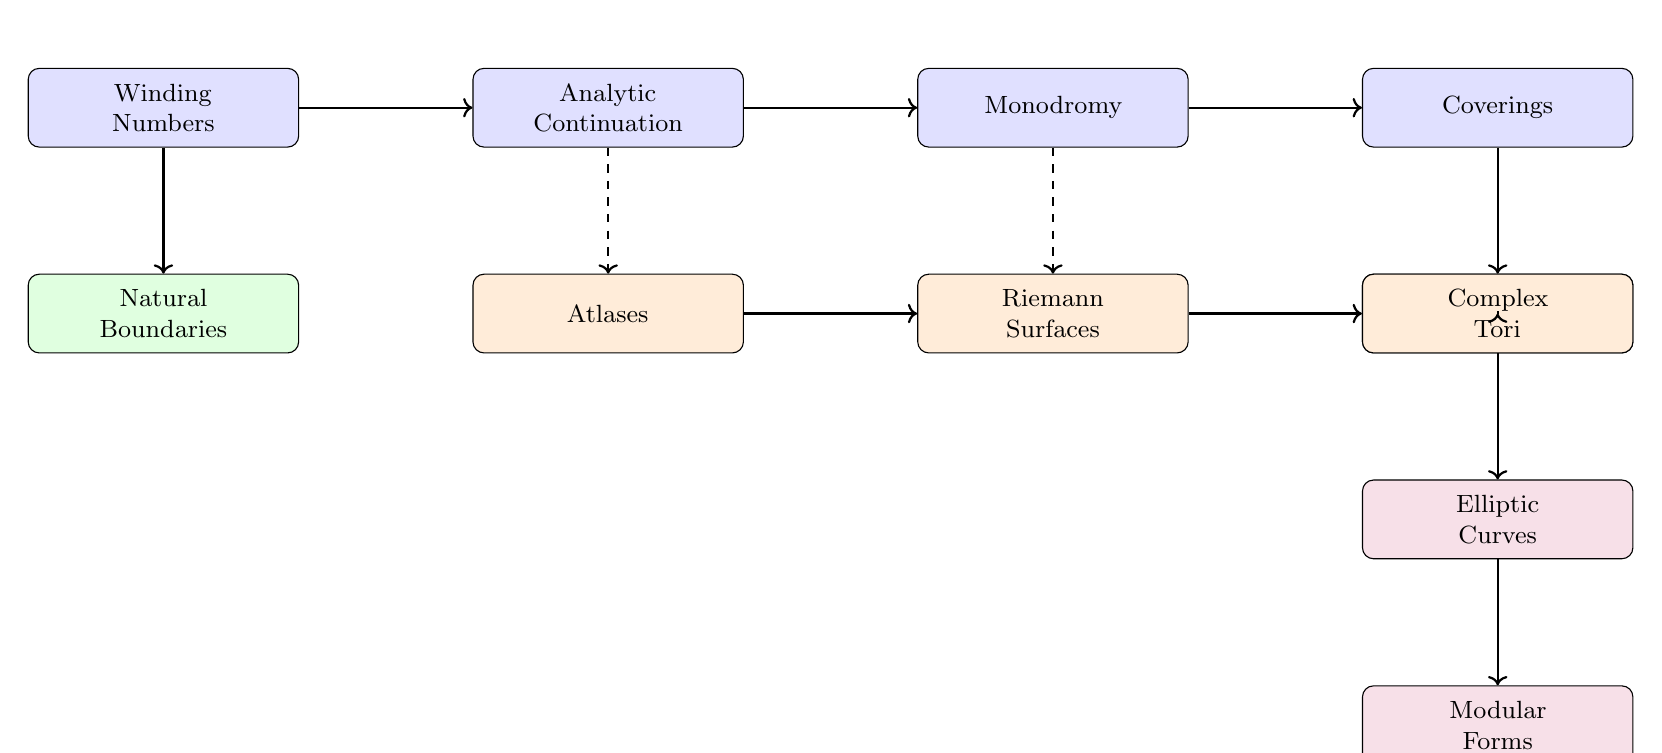
\begin{tikzpicture}[
			node distance=1.6cm and 2.2cm,
			every node/.style={
				draw,
				rounded corners,
				align=center,
				text width=3.2cm,
				minimum height=1cm,
				font=\small
			},
			main/.style={fill=blue!12},
			side/.style={fill=green!12},
			deep/.style={fill=orange!15},
			final/.style={fill=purple!12},
			arrow/.style={->,thick}
			]
			
			\node[main] (wind) {Winding\\Numbers};
			\node[main,right=of wind] (cont) {Analytic\\Continuation};
			\node[main,right=of cont] (mono) {Monodromy};
			\node[main,right=of mono] (cov) {Coverings};
			
			\node[side,below=of wind] (bound) {Natural\\Boundaries};
			\node[side,below=of cov] (deck) {Deck\\Transformations};
			
			\node[deep,below=of cont] (atl) {Atlases};
			\node[deep,right=of atl] (rs) {Riemann\\Surfaces};
			\node[deep,right=of rs] (torus) {Complex\\Tori};
			
			\node[final,below=of torus] (ell) {Elliptic\\Curves};
			\node[final,below=of ell] (mod) {Modular\\Forms};
			
			\draw[arrow] (wind) -- (cont);
			\draw[arrow] (cont) -- (mono);
			\draw[arrow] (mono) -- (cov);
			
			\draw[arrow] (wind) -- (bound);
			\draw[arrow] (cov) -- (deck);
			
			\draw[arrow] (deck) -- (torus);
			\draw[arrow] (atl) -- (rs);
			\draw[arrow] (rs) -- (torus);
			
			\draw[arrow] (torus) -- (ell);
			\draw[arrow] (ell) -- (mod);
			
			\draw[arrow,dashed] (cont) -- (atl);
			\draw[arrow,dashed] (mono) -- (rs);
			
		\end{tikzpicture}
	}
\end{center}

Thus Problems~1--9 form a miniature introduction to the modern theory of

\[
\boxed{
	\begin{gathered}
		\text{Riemann Surfaces},\quad
		\text{Covering Spaces},\quad
		\text{Elliptic Functions},\\
		\text{Complex Tori},\quad
		\text{Algebraic Curves},\quad
		\text{Modular Forms}.
	\end{gathered}
}
\]

\section{Problem 10: A Quotient of \texorpdfstring{$\mathbb C^\ast$}{C*} as a Complex Torus}

\subsection*{Statement}

Define an equivalence relation on

\[
\mathbb C^\ast=\mathbb C\setminus\{0\}
\]

by

\[
z\sim w
\]

if

\[
z=2^s w
\]

for some

\[
s\in\mathbb Z.
\]

Show that the quotient space

\[
R=\mathbb C^\ast/\sim
\]

has the natural structure of a compact Riemann surface, and that \(R\) is analytically isomorphic to a complex torus.

\subsection*{Solution}

The key idea is to convert multiplication into addition using the logarithm.

\subsubsection*{Step 1: Pass to the Universal Covering}

Recall that

\[
\exp:\mathbb C\to\mathbb C^\ast
\]

is the universal covering map.

Write

\[
z=e^u.
\]

The relation

\[
z\sim 2^s z
\]

becomes

\[
e^u
\sim
e^{u+s\log 2}.
\]

Since

\[
e^{u+2\pi i k}=e^u,
\qquad
k\in\mathbb Z,
\]

the coordinate \(u\) is identified by

\[
u
\sim
u+s\log 2+2\pi i k,
\qquad
s,k\in\mathbb Z.
\]

Thus the quotient can be written as

\[
R
\cong
\mathbb C/
\langle
\log 2,
2\pi i
\rangle.
\]

\subsubsection*{Step 2: The Associated Lattice}

Define

\[
\Lambda
=
\langle
\log 2,
2\pi i
\rangle.
\]

Since

\[
\log 2
\]

and

\[
2\pi i
\]

are linearly independent over \(\mathbb R\),

\[
\Lambda
\]

is a lattice in \(\mathbb C\).

Hence

\[
\mathbb C/\Lambda
\]

is a complex torus.

Therefore

\[
R
\cong
\mathbb C/\Lambda.
\]

\subsubsection*{Step 3: Compactness}

A fundamental parallelogram for the lattice is

\[
P
=
\{
a\log2+b(2\pi i):
0\le a,b<1
\}.
\]

Every equivalence class has a representative in \(P\).

Since \(P\) is compact, the quotient

\[
\mathbb C/\Lambda
\]

is compact.

Hence

\[
R
\]

is compact.

\subsubsection*{Step 4: Complex Structure}

Translations

\[
u\mapsto u+\lambda,
\qquad
\lambda\in\Lambda,
\]

are holomorphic maps.

Therefore the quotient inherits a natural complex structure.

Hence

\[
R
\]

is a compact Riemann surface.

\subsection*{Conclusion}

\[
\boxed{
	R
	=
	\mathbb C^\ast/\{z\sim2^s z\}
	\cong
	\mathbb C/
	\langle\log2,2\pi i\rangle.
}
\]

Therefore

\[
\boxed{
	R
	\text{ is a compact Riemann surface and a complex torus.}
}
\]

\bigskip

\section{Problem 11: Identity Principle for Riemann Surfaces}

\subsection*{Statement}

Let \(R,S\) be Riemann surfaces and let

\[
f,g:R\to S
\]

be analytic maps.

Define

\[
E
=
\{z\in R:f(z)=g(z)\}.
\]

Show that either

\[
E=R
\]

or \(E\) contains only isolated points.

\subsection*{Solution}

The proof is local and reduces the statement to the classical identity theorem for holomorphic functions.

Let

\[
p\in E.
\]

Then

\[
f(p)=g(p).
\]

Choose charts

\[
(U,\phi)
\]

around \(p\) and

\[
(V,\psi)
\]

around

\[
f(p)=g(p).
\]

Define local representatives

\[
F
=
\psi\circ f\circ\phi^{-1},
\qquad
G
=
\psi\circ g\circ\phi^{-1}.
\]

These are holomorphic functions on an open subset of \(\mathbb C\).

The set \(E\) corresponds locally to

\[
\{w:F(w)=G(w)\}.
\]

Define

\[
H(w)=F(w)-G(w).
\]

Then \(H\) is holomorphic.

\subsubsection*{Case 1: \(H\equiv0\)}

If

\[
H\equiv0,
\]

then

\[
F=G
\]

on the chart.

Therefore

\[
f=g
\]

on a neighborhood of \(p\).

By analytic continuation and connectedness of \(R\),

\[
f=g
\]

everywhere on \(R\).

Hence

\[
E=R.
\]

\subsubsection*{Case 2: \(H\not\equiv0\)}

If \(H\) is not identically zero, then the classical identity theorem implies that its zeros are isolated.

Consequently

\[
\{H=0\}
\]

consists only of isolated points.

Thus \(E\) contains only isolated points.

\subsection*{Conclusion}

Exactly one of the following alternatives holds:

\[
\boxed{
	E=R,
}
\]

or

\[
\boxed{
	E
	\text{ consists entirely of isolated points.}
}
\]

This is the identity principle for Riemann surfaces.

\bigskip

\section{Problem 12: Harmonic Functions and Holomorphic Functions}

\subsection*{Statement}

Let

\[
D\subset\mathbb C
\]

be an open disc and let

\[
u:D\to\mathbb R
\]

be harmonic.

Define

\[
g=u_x-i u_y.
\]

Show that \(g\) is analytic.

If \(z_0\) denotes the center of the disc, define

\[
f(z)
=
u(z_0)
+
\int_{z_0}^{z}
g(t)\,dt,
\]

where the integral is taken along the straight line segment from \(z_0\) to \(z\).

Show that \(f\) is analytic with

\[
f'=g,
\]

and that

\[
u=\operatorname{Re}(f).
\]

\subsection*{Solution}

Since \(u\) is harmonic,

\[
u_{xx}+u_{yy}=0.
\]

Define

\[
g=u_x-i u_y.
\]

Write

\[
g=P+iQ,
\]

where

\[
P=u_x,
\qquad
Q=-u_y.
\]

We verify the Cauchy--Riemann equations.

\subsubsection*{First Cauchy--Riemann Equation}

We have

\[
P_x=u_{xx}.
\]

Also,

\[
Q_y=-u_{yy}.
\]

Since

\[
u_{xx}+u_{yy}=0,
\]

it follows that

\[
P_x=Q_y.
\]

\subsubsection*{Second Cauchy--Riemann Equation}

We have

\[
P_y=u_{xy},
\]

and

\[
Q_x=-u_{yx}.
\]

Since mixed partial derivatives commute,

\[
u_{xy}=u_{yx},
\]

we obtain

\[
P_y=-Q_x.
\]

Thus the Cauchy--Riemann equations hold.

Therefore

\[
\boxed{
	g=u_x-i u_y
}
\]

is holomorphic on \(D\).

\subsection*{Constructing the Holomorphic Function}

Define

\[
f(z)
=
u(z_0)
+
\int_{z_0}^{z}
g(t)\,dt.
\]

Since \(g\) is holomorphic and \(D\) is simply connected, Cauchy's theorem implies that the integral is path independent.

Therefore \(f\) is well defined.

By the fundamental theorem of complex integration,

\[
\boxed{
	f'(z)=g(z).
}
\]

\subsection*{Showing that \(u=\Re(f)\)}

Write

\[
f=u+iv.
\]

Then

\[
f'
=
u_x+i v_x.
\]

Since

\[
f'
=
g
=
u_x-i u_y,
\]

we obtain

\[
v_x=-u_y.
\]

Comparing imaginary parts gives

\[
v_y=u_x.
\]

These are precisely the Cauchy--Riemann equations.

Hence \(u\) and \(v\) form a harmonic conjugate pair.

Since

\[
f(z_0)=u(z_0),
\]

the additive constant is chosen correctly.

Therefore

\[
\boxed{
	u=\operatorname{Re}(f).
}
\]

\subsection*{Interpretation}

This result establishes one of the fundamental correspondences of complex analysis:

\[
\boxed{
	\text{Harmonic Functions}
	\Longleftrightarrow
	\text{Real Parts of Holomorphic Functions}.
}
\]

The function

\[
v=\operatorname{Im}(f)
\]

is called a \emph{harmonic conjugate} of \(u\).

The holomorphic function

\[
f=u+iv
\]

is the analytic function associated with the harmonic function \(u\).

Thus every harmonic function on a disc arises as the real part of a holomorphic function.
	
\section{Problem 13: Coincidence Sets of Harmonic Functions}

\subsection*{Statement}

Suppose \(u,v\) are harmonic functions on a Riemann surface \(R\), and let

\[
E
=
\{z\in R : u(z)=v(z)\}.
\]

Show that either

\[
E=R,
\]

or \(E\) has empty interior.

Give an example showing that \(E\) does not in general consist of isolated points.

\subsection*{Solution}

Define

\[
w=u-v.
\]

Since both \(u\) and \(v\) are harmonic,

\[
\Delta w
=
\Delta u-\Delta v
=
0.
\]

Therefore \(w\) is harmonic.

Observe that

\[
E
=
\{z\in R:w(z)=0\}.
\]

Thus \(E\) is the zero set of the harmonic function \(w\).

\subsubsection*{Step 1: Suppose \(E\) Contains an Open Set}

Assume there exists a nonempty open subset

\[
U\subset E.
\]

Then

\[
w=0
\]

on \(U\).

Since harmonic functions are real analytic, the identity theorem for real analytic functions implies that a harmonic function vanishing on a nonempty open set must vanish identically on the connected component containing that set.

Hence

\[
w\equiv0.
\]

Therefore

\[
u=v
\]

everywhere on \(R\).

Consequently

\[
E=R.
\]

\subsubsection*{Step 2: Contrapositive}

If

\[
E\neq R,
\]

then \(w\) is not identically zero.

A nonzero harmonic function cannot vanish on any nonempty open set.

Therefore

\[
\operatorname{Int}(E)=\varnothing.
\]

Thus

\[
\boxed{
	E=R
	\quad\text{or}\quad
	E\text{ has empty interior.}
}
\]

\subsection*{Example Showing that \(E\) Need Not Consist of Isolated Points}

Let

\[
R=\mathbb C.
\]

Define

\[
u(x+iy)=x,
\qquad
v(x+iy)=0.
\]

Both functions are harmonic because

\[
\Delta u=0,
\qquad
\Delta v=0.
\]

Then

\[
E
=
\{z:u(z)=v(z)\}
=
\{x=0\}.
\]

Hence

\[
E=i\mathbb R.
\]

This set is an entire line.

Every point of \(E\) is an accumulation point of \(E\).

Therefore \(E\) does not consist of isolated points.

However,

\[
\operatorname{Int}(E)=\varnothing.
\]

Thus

\[
\boxed{
	E=i\mathbb R
}
\]

provides the required example.

\bigskip

\section{Problem 14: Four-Punctured Spheres and Cross-Ratios}

\subsection*{Statement}

Let

\[
\{a_1,a_2,a_3,a_4\}
\]

and

\[
\{b_1,b_2,b_3,b_4\}
\]

be sets of four distinct points of

\[
\widehat{\mathbb C}.
\]

Show that every analytic isomorphism

\[
f:
\widehat{\mathbb C}
\setminus
\{a_1,a_2,a_3,a_4\}
\longrightarrow
\widehat{\mathbb C}
\setminus
\{b_1,b_2,b_3,b_4\}
\]

extends to an analytic isomorphism

\[
\widehat{\mathbb C}
\longrightarrow
\widehat{\mathbb C}.
\]

Using this result, find a necessary and sufficient condition for

\[
\mathbb C\setminus\{0,1,a\}
\]

to be conformally equivalent to

\[
\mathbb C\setminus\{0,1,b\},
\]

where

\[
a,b\neq0,1.
\]

\subsection*{Solution}

\subsubsection*{Step 1: Extension Across the Punctures}

Consider a puncture

\[
a_i.
\]

Since \(f\) is a biholomorphism between punctured compact Riemann surfaces, the singularity of \(f\) at \(a_i\) cannot be essential.

Indeed, by the Casorati--Weierstrass theorem (or Picard's theorem), an essential singularity would force the image of a punctured neighborhood to be dense in the sphere, contradicting injectivity.

The singularity cannot be a pole either, because the inverse map would fail to extend holomorphically.

Therefore every puncture is removable.

Hence \(f\) extends holomorphically across all four punctures.

We obtain a holomorphic map

\[
F:\widehat{\mathbb C}\to\widehat{\mathbb C}.
\]

Applying the same argument to \(f^{-1}\), we see that \(F^{-1}\) is also holomorphic.

Thus \(F\) is a biholomorphic automorphism of the Riemann sphere.

\subsubsection*{Step 2: Automorphisms of the Sphere}

The automorphisms of

\[
\widehat{\mathbb C}
\]

are precisely the Möbius transformations

\[
F(z)
=
\frac{az+b}{cz+d},
\qquad
ad-bc\neq0.
\]

Therefore

\[
\boxed{
	f
	\text{ extends uniquely to a Möbius transformation.}
}
\]

\subsection*{Cross-Ratios}

For four points

\[
(z_1,z_2,z_3,z_4)
\]

their cross-ratio is

\[
[z_1,z_2;z_3,z_4]
=
\frac{(z_1-z_3)(z_2-z_4)}
{(z_1-z_4)(z_2-z_3)}.
\]

A fundamental theorem states that Möbius transformations preserve cross-ratios.

Thus the conformal type of a four-punctured sphere is determined by the cross-ratio of its punctures.

\subsection*{Application to \(\mathbb C\setminus\{0,1,a\}\)}

Write

\[
\mathbb C\setminus\{0,1,a\}
=
\widehat{\mathbb C}
\setminus
\{\infty,0,1,a\}.
\]

The cross-ratio of the four points

\[
(\infty,0,1,a)
\]

is

\[
[\infty,0;1,a].
\]

Using the standard simplification when one point is infinity,

\[
[\infty,0;1,a]
=
\frac{0-a}{0-1}
=
a.
\]

Hence the conformal type is determined by \(a\).

However, permuting the four punctures produces the six equivalent cross-ratio values

\[
a,
\qquad
1-a,
\qquad
\frac1a,
\qquad
\frac1{1-a},
\qquad
\frac{a-1}{a},
\qquad
\frac{a}{a-1}.
\]

These are exactly the values obtained from all permutations of the four points.

\subsection*{Conclusion}

Therefore

\[
\mathbb C\setminus\{0,1,a\}
\]

and

\[
\mathbb C\setminus\{0,1,b\}
\]

are conformally equivalent if and only if

\[
b
\]

belongs to the six-element orbit

\[
\boxed{
	\left\{
	a,
	\;
	1-a,
	\;
	\frac1a,
	\;
	\frac1{1-a},
	\;
	\frac{a-1}{a},
	\;
	\frac{a}{a-1}
	\right\}.
}
\]

Equivalently,

\[
\boxed{
	\mathbb C\setminus\{0,1,a\}
	\cong
	\mathbb C\setminus\{0,1,b\}
}
\]

if and only if \(a\) and \(b\) determine the same cross-ratio up to permutation of the punctures.	
	
\section{Theory Behind Problems 13--14:
	Harmonic Functions, Identity Principles, and Moduli of Four-Pointed Spheres}

Problems~13 and~14 continue the development of the theory of Riemann surfaces in two complementary directions.

The first concerns the relationship between harmonic and holomorphic functions:

\[
\boxed{
	\text{Harmonic Functions}
	\Longrightarrow
	\text{Holomorphic Functions}
	\Longrightarrow
	\text{Identity Principles}
}
\]

while the second concerns the geometry of punctured spheres:

\[
\boxed{
	\text{Möbius Transformations}
	\Longrightarrow
	\text{Cross-Ratios}
	\Longrightarrow
	\text{Moduli Spaces}
}
\]

Together these topics form the bridge between classical complex analysis and modern algebraic geometry.

\bigskip

\subsection{1. Harmonic Functions on Riemann Surfaces}

Let

\[
R
\]

be a Riemann surface.

A function

\[
u:R\to\mathbb R
\]

is called \emph{harmonic} if in every local coordinate

\[
z=x+iy
\]

it satisfies Laplace's equation

\[
\Delta u
=
u_{xx}+u_{yy}
=
0.
\]

The operator

\[
\Delta
=
\frac{\partial^2}{\partial x^2}
+
\frac{\partial^2}{\partial y^2}
\]

is called the Laplacian.

\subsubsection*{Physical Interpretation}

Harmonic functions occur naturally in:

\begin{itemize}
	\item Electrostatic potentials,
	\item Gravitational potentials,
	\item Steady-state heat distributions,
	\item Incompressible fluid flow,
	\item Minimal surfaces.
\end{itemize}

Thus harmonic functions arise throughout mathematics and physics.

\bigskip

\subsection{2. Harmonic Functions are Real Analytic}

One of the deepest properties of harmonic functions is:

\begin{theorem}
	Every harmonic function is real analytic.
\end{theorem}

Consequently every harmonic function admits a convergent power series expansion

\[
u(x,y)
=
\sum_{m,n\ge0}
a_{mn}
(x-x_0)^m
(y-y_0)^n.
\]

This property is much stronger than smoothness.

In particular, harmonic functions satisfy an identity theorem analogous to that for holomorphic functions.

\bigskip

\subsection{3. Identity Principle for Harmonic Functions}

Suppose

\[
u,v
\]

are harmonic.

Define

\[
w=u-v.
\]

Then \(w\) is harmonic.

If

\[
u=v
\]

on a nonempty open set, then

\[
w=0
\]

on a nonempty open set.

Since \(w\) is real analytic,

\[
w\equiv0.
\]

Therefore

\[
u=v
\]

everywhere on the connected component.

Hence:

\[
\boxed{
	\text{Two harmonic functions that agree on an open set are identical.}
}
\]

This is the fundamental principle used in Problem~13.

\bigskip

\subsection{4. Difference from Holomorphic Functions}

For holomorphic functions:

\[
f=g
\]

on a set with an accumulation point implies

\[
f=g.
\]

The coincidence set is either the whole domain or consists of isolated points.

For harmonic functions this is no longer true.

The coincidence set may contain entire curves.

For example,

\[
u(x,y)=x,
\qquad
v(x,y)=0.
\]

Then

\[
u=v
\]

precisely on

\[
x=0.
\]

Thus the coincidence set is

\[
i\mathbb R,
\]

the entire imaginary axis.

Hence

\[
\boxed{
	\text{Coincidence sets of harmonic functions may contain curves.}
}
\]

This is the key distinction between Problems~11 and~13.

\bigskip

\subsection{5. Geometry of Zero Sets of Harmonic Functions}

The local structure of harmonic functions near zeros is remarkably regular.

If

\[
u
=
\operatorname{Re}(z^n)
\]

then

\[
u=0
\]

consists of \(2n\) rays meeting at equal angles.

Examples:

\[
\operatorname{Re}(z)
=
x
\]

has zero set

\[
x=0.
\]

\[
\operatorname{Re}(z^2)
=
x^2-y^2
\]

has zero set

\[
y=\pm x.
\]

\[
\operatorname{Re}(z^3)
=
x^3-3xy^2
\]

has six rays meeting at angles of

\[
60^\circ.
\]

In general, near a zero of order \(n\),

\[
u
=
\operatorname{Re}(z^n)+\cdots,
\]

and the nodal set consists of

\[
2n
\]

smooth arcs meeting equally.

Thus harmonic functions naturally generate geometric networks.

\bigskip

\subsection{6. Harmonic Conjugates}

Problem~12 established that if

\[
u
\]

is harmonic on a simply connected domain, then there exists a harmonic conjugate

\[
v
\]

such that

\[
f=u+iv
\]

is holomorphic.

The pair \((u,v)\) satisfies the Cauchy--Riemann equations:

\[
u_x=v_y,
\qquad
u_y=-v_x.
\]

Consequently

\[
\boxed{
	\text{Harmonic Functions}
	\Longleftrightarrow
	\text{Real Parts of Holomorphic Functions}.
}
\]

This relationship lies at the heart of complex analysis.

\bigskip

\subsection{7. The Riemann Sphere and Möbius Transformations}

Problem~14 concerns the geometry of

\[
\widehat{\mathbb C}
=
\mathbb C\cup\{\infty\}.
\]

This space is called the \emph{Riemann sphere}.

Its automorphism group is

\[
\operatorname{Aut}(\widehat{\mathbb C})
=
PSL(2,\mathbb C).
\]

Every automorphism has the form

\[
z
\mapsto
\frac{az+b}{cz+d},
\qquad
ad-bc\neq0.
\]

These maps are called Möbius transformations.

\bigskip

\subsection{8. Three Points Determine a Möbius Transformation}

A fundamental theorem states:

\begin{theorem}
	Given distinct points
	
	\[
	a,b,c
	\]
	
	and
	
	\[
	A,B,C,
	\]
	
	there exists a unique Möbius transformation satisfying
	
	\[
	a\mapsto A,
	\qquad
	b\mapsto B,
	\qquad
	c\mapsto C.
	\]
\end{theorem}

Therefore every triple of distinct points may be normalized to

\[
0,\quad1,\quad\infty.
\]

This explains why three marked points on a sphere carry no moduli.

\bigskip

\subsection{9. Why Four Points are Different}

After fixing

\[
0,\quad1,\quad\infty,
\]

a fourth point remains.

Its position cannot be removed by a Möbius transformation.

Thus a sphere with four marked points possesses one complex parameter.

This parameter is the cross-ratio.

\bigskip

\subsection{10. Cross-Ratios}

For four distinct points

\[
(z_1,z_2,z_3,z_4)
\]

define

\[
[z_1,z_2;z_3,z_4]
=
\frac{(z_1-z_3)(z_2-z_4)}
{(z_1-z_4)(z_2-z_3)}.
\]

The cross-ratio is invariant under Möbius transformations:

\[
[M(z_1),M(z_2);M(z_3),M(z_4)]
=
[z_1,z_2;z_3,z_4].
\]

Therefore it is the fundamental invariant of four-point configurations on the sphere.

\bigskip

\subsection{11. The Moduli Space of Four Points}

Every quadruple of distinct points can be transformed into

\[
(\infty,0,1,\lambda).
\]

The parameter

\[
\lambda
\]

determines the conformal type.

However permutations of the four points produce six equivalent values:

\[
\lambda,
\qquad
1-\lambda,
\qquad
\frac1\lambda,
\qquad
\frac1{1-\lambda},
\qquad
\frac{\lambda-1}{\lambda},
\qquad
\frac{\lambda}{\lambda-1}.
\]

Hence

\[
\boxed{
	\mathcal M_{0,4}
	=
	(\mathbb C\setminus\{0,1\})/S_3.
}
\]

This is the moduli space of four-pointed spheres.

Problem~14 computes precisely this equivalence relation.

\bigskip

\subsection{12. Connection with Elliptic Curves}

The theory becomes even richer when one considers

\[
y^2
=
x(x-1)(x-\lambda).
\]

The branch points are

\[
0,\quad1,\quad\lambda,\quad\infty.
\]

The associated Riemann surface is a torus.

Thus the parameter

\[
\lambda
\]

controls the complex structure of an elliptic curve.

This family is called the \emph{Legendre family}.

Consequently

\[
\boxed{
	\text{Cross-Ratios}
	\Longrightarrow
	\text{Elliptic Curves}.
}
\]

\bigskip

\subsection{13. Modular Functions}

Every complex torus can be written as

\[
T_\tau
=
\mathbb C/\langle1,\tau\rangle.
\]

The Legendre parameter and the torus parameter are related by

\[
\lambda
=
\lambda(\tau),
\]

where \(\lambda(\tau)\) is the modular lambda function.

Hence

\[
\boxed{
	\text{Four-Pointed Spheres}
	\Longleftrightarrow
	\text{Complex Tori}.
}
\]

This connection is one of the foundations of modern algebraic geometry.

\bigskip

\subsection{Grand Synthesis}

The conceptual flow behind Problems~13--14 is

\[
\boxed{
	\text{Harmonic Functions}
	\Longrightarrow
	\text{Holomorphic Functions}
	\Longrightarrow
	\text{Identity Principles}
}
\]

and simultaneously

\[
\boxed{
	\text{Möbius Transformations}
	\Longrightarrow
	\text{Cross-Ratios}
	\Longrightarrow
	\text{Moduli Spaces}
}
\]

which ultimately leads to

\[
\boxed{
	\text{Cross-Ratios}
	\Longrightarrow
	\text{Elliptic Curves}
	\Longrightarrow
	\text{Complex Tori}
	\Longrightarrow
	\text{Modular Forms}.
}
\]

Thus Problems~13--14 mark the transition from classical complex analysis to the modern theory of moduli spaces, elliptic curves, and algebraic geometry.	
	
\end{document}

